\chapter{栈、队列和数组}\label{DS03}

\section{栈与合法出栈序列}\label{DS03-stack}

栈只允许在栈顶插入、删除，遵循后进先出。空栈不能出栈，固定容量满栈不能入栈。

检验输出序列：按目标输出依次处理；当前栈顶不符时继续按输入次序入栈，到目标位于栈顶时弹出。输入耗尽且栈顶仍不符即失败。模拟期间最大栈深为实现该输出所需的最小容量。

从空栈出发并回到空栈的合法入出操作序列满足：入栈与出栈总数相同，每个前缀中出栈数不超过入栈数。\(n\)个不同元素的合法出栈序列数为

\[C_n=\frac1{n+1}\binom{2n}{n}.\]

\par\medskip\Needspace{4\baselineskip}\noindent\hypertarget{DS03-E01}{}\label{DS03-E01}\textbf{例 3-1}\par\nobreak\smallskip

栈 \(S\) 和队列 \(Q\) 初始均为空，元素 \texttt{a,\allowbreak{}b,\allowbreak{}c,\allowbreak{}d,\allowbreak{}e,\allowbreak{}f,\allowbreak{}g} 依次入栈 \(S\)。每个元素出栈后立即进入队列 \(Q\)，7个元素出队顺序为 \texttt{b,\allowbreak{}d,\allowbreak{}c,\allowbreak{}f,\allowbreak{}e,\allowbreak{}a,\allowbreak{}g}，则栈容量至少是（　）。

A. 1　B. 2　C. 3　D. 4

\subsection{顺序栈与共享栈}\label{DS03-stack-code}

顺序栈下标从0开始，\texttt{top}指当前栈顶，空时为\ensuremath{-}1。

\par\smallskip\noindent\begin{minipage}{\linewidth}
\begin{codeblock}[language={C++}]
#define MaxSize 100
typedef int ElemType;
typedef struct {
    ElemType data[MaxSize];
    int top;
} SqStack;
void InitStack(SqStack &S) { S.top = -1; }
bool StackEmpty(SqStack S) { return S.top == -1; }
bool Push(SqStack &S, ElemType x) {
    if (S.top == MaxSize - 1) return false;
    S.data[++S.top] = x;
    return true;
}
bool Pop(SqStack &S, ElemType &x) {
    if (S.top == -1) return false;
    x = S.data[S.top--];
    return true;
}
bool GetTop(SqStack S, ElemType &x) {
    if (S.top == -1) return false;
    x = S.data[S.top];
    return true;
}
\end{codeblock}
\end{minipage}\par\smallskip

若\texttt{top}改指下一空位，须同时改为空时0、入栈\texttt{data[\allowbreak{}top+\allowbreak{}+\allowbreak{}]\allowbreak{}=\allowbreak{}x}、出栈\texttt{x=\allowbreak{}data[\allowbreak{}--top]\allowbreak{}}。

共享栈从同一数组两端向中间增长。教材\texttt{ShStack}采用如下初值：

\par\smallskip\noindent\begin{minipage}{\linewidth}
\begin{codeblock}[language={C++}]
typedef struct {
    ElemType data[MaxSize];
    int top0, top1;
} ShStack;
void InitStack(ShStack &S) {
    S.top0 = -1;
    S.top1 = MaxSize;
}
\end{codeblock}
\end{minipage}\par\smallskip

\par\smallskip
{\fontsize{9.3}{12}\selectfont\setlength{\tabcolsep}{2.5pt}\setlength{\LTleft}{0pt}\setlength{\LTright}{0pt}
\begin{longtable}{@{}>{\raggedright\arraybackslash}p{\dimexpr0.27041\linewidth-2\tabcolsep\relax}>{\raggedright\arraybackslash}p{\dimexpr0.36480\linewidth-2\tabcolsep\relax}>{\raggedright\arraybackslash}p{\dimexpr0.36480\linewidth-2\tabcolsep\relax}@{}}
\toprule
操作 & 0号栈 & 1号栈 \\

\midrule\endfirsthead\toprule
操作 & 0号栈 & 1号栈 \\

\midrule\endhead\bottomrule\endfoot
判空 & \texttt{top0==-1} & \texttt{top1==MaxSize} \\

入栈 & \texttt{data{[}++top0{]}=x} & \texttt{data{[}-\/-top1{]}=x} \\

出栈 & \texttt{x=data{[}top0-\/-{]}} & \texttt{x=data{[}top1++{]}} \\

\end{longtable}}
\par\smallskip

两栈共用的满条件为\texttt{top1-top0=\allowbreak{}=\allowbreak{}1}。入栈先判满，出栈先判各自是否为空。

\subsection{链栈}\label{DS03-linked-stack}

链栈通常无头结点，以链头为栈顶，初始化\texttt{S=\allowbreak{}NULL}。头插、头删均为\(O(1)\)；入栈可能因申请失败而失败。

\par\smallskip\noindent\begin{minipage}{\linewidth}
\begin{codeblock}[language={C++}]
typedef struct Linknode {
    ElemType data;
    struct Linknode *next;
} *LiStack;
bool Push(LiStack &S, ElemType x) {
    LiStack p = (LiStack)malloc(sizeof(struct Linknode));
    if (p == NULL) return false;
    p->data = x;
    p->next = S;
    S = p;
    return true;
}
bool Pop(LiStack &S, ElemType &x) {
    if (S == NULL) return false;
    LiStack p = S;
    x = p->data;
    S = p->next;
    free(p);
    return true;
}
\end{codeblock}
\end{minipage}\par\smallskip

\section{队列、双端队列与循环表示}\label{DS03-queue}

队列在队尾插入、队头删除，先进先出。双端队列允许两端插入和删除；输入受限版本只允许一端输入，输出受限版本只允许一端输出。两种受限模型须分别模拟。

按1、2、3、4顺序输入，输入受限双端队列有22种输出，不能得到\texttt{4,\allowbreak{}2,\allowbreak{}1,\allowbreak{}3}及\texttt{4,\allowbreak{}2,\allowbreak{}3,\allowbreak{}1}；输出受限双端队列有22种输出，不能得到\texttt{4,\allowbreak{}1,\allowbreak{}3,\allowbreak{}2}及\texttt{4,\allowbreak{}2,\allowbreak{}3,\allowbreak{}1}。普通栈有14种输出。

循环队列采用长度\(M\)的数组，\texttt{front}指队头，\texttt{rear}指下一入队位置。入队后推进\texttt{rear}，出队后推进\texttt{front}，均对\(M\)取模。

\par\smallskip
\begin{wideblock}
{\fontsize{9.3}{12}\selectfont\setlength{\tabcolsep}{2.5pt}\setlength{\LTleft}{0pt}\setlength{\LTright}{0pt}
\begin{longtable}{@{}>{\raggedright\arraybackslash}p{\dimexpr0.23910\linewidth-2\tabcolsep\relax}>{\raggedright\arraybackslash}p{\dimexpr0.27942\linewidth-2\tabcolsep\relax}>{\raggedright\arraybackslash}p{\dimexpr0.27942\linewidth-2\tabcolsep\relax}>{\raggedright\arraybackslash}p{\dimexpr0.20207\linewidth-2\tabcolsep\relax}@{}}
\toprule
区分空满的方法 & 空 & 满 & 最大元素数 \\

\midrule\endfirsthead\toprule
区分空满的方法 & 空 & 满 & 最大元素数 \\

\midrule\endhead\bottomrule\endfoot
牺牲一单元 & \texttt{front==rear} & \texttt{(rear+1)\%M==front} & \(M-1\) \\

增加\texttt{size} & \texttt{size==0} & \texttt{size==M} & \(M\) \\

最近操作\texttt{tag} & 指针相同且tag为出队 & 指针相同且tag为入队 & \(M\) \\

\end{longtable}}
\end{wideblock}
\par\smallskip

\texttt{tag}初始为出队态，成功操作后才更新。牺牲单元方案长度为

\[len=(rear-front+M)\bmod M.\]

\par\smallskip\noindent\begin{minipage}{\linewidth}
\begin{codeblock}[language={C++}]
typedef struct {
    ElemType data[MaxSize];
    int front, rear;
} SqQueue;
void InitQueue(SqQueue &Q) { Q.front = Q.rear = 0; }
bool QueueEmpty(SqQueue Q) { return Q.front == Q.rear; }
bool EnQueue(SqQueue &Q, ElemType x) {
    if ((Q.rear + 1) % MaxSize == Q.front) return false;
    Q.data[Q.rear] = x;
    Q.rear = (Q.rear + 1) % MaxSize;
    return true;
}
bool DeQueue(SqQueue &Q, ElemType &x) {
    if (Q.front == Q.rear) return false;
    x = Q.data[Q.front];
    Q.front = (Q.front + 1) % MaxSize;
    return true;
}
bool GetHead(SqQueue Q, ElemType &x) {
    if (Q.front == Q.rear) return false;
    x = Q.data[Q.front];
    return true;
}
\end{codeblock}
\end{minipage}\par\smallskip

\begin{figure}
\centering
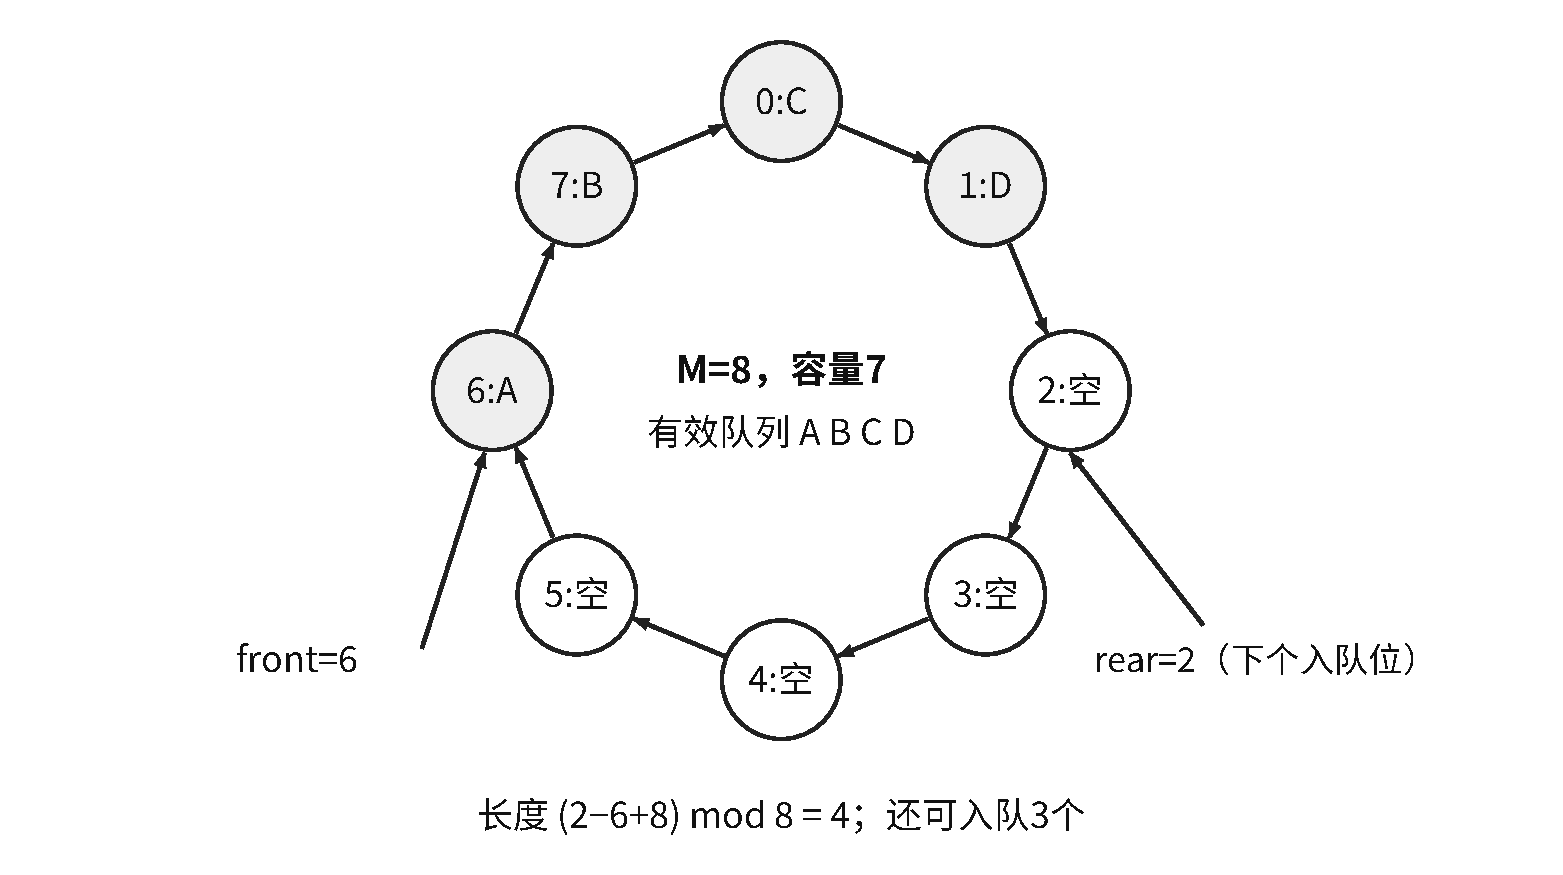
\includegraphics[width=\linewidth,height=108mm,keepaspectratio]{figures/DS_03_circular_queue.pdf}
\caption{循环队列的环绕与空满状态}\label{DS03-circular-figure}
\end{figure}

\par\medskip\Needspace{4\baselineskip}\noindent\hypertarget{DS03-E02}{}\label{DS03-E02}\textbf{例 3-2}\par\nobreak\smallskip

循环队列存于数组 \texttt{A[\allowbreak{}21]\allowbreak{}}，\texttt{front} 指向队首元素的前一个位置，\texttt{rear} 指向队尾元素。当前 \texttt{front=\allowbreak{}8,\allowbreak{} rear=\allowbreak{}3}，队列长度为（　）。

A. 5　B. 6　C. 16　D. 17

若\texttt{front}指队头、\texttt{rear}指当前队尾，可令空状态\texttt{front=\allowbreak{}0,\allowbreak{}rear=\allowbreak{}M-1}；入队先推进\texttt{rear}再写，出队先取后推进\texttt{front}。牺牲一单元时空条件\texttt{(\allowbreak{}rear+\allowbreak{}1)\allowbreak{}\%M=\allowbreak{}=\allowbreak{}front}、满条件\texttt{(\allowbreak{}rear+\allowbreak{}2)\allowbreak{}\%M=\allowbreak{}=\allowbreak{}front}，长度\texttt{(\allowbreak{}rear-front+\allowbreak{}1+\allowbreak{}M)\allowbreak{}\%M}。数组\texttt{A[\allowbreak{}0.\allowbreak{}.\allowbreak{}n]\allowbreak{}}共有\(n+1\)单元，模数须取\(n+1\)。

\subsection{链队列}\label{DS03-linked-queue}

单链队列以链头为队头、链尾为队尾，保存\texttt{front、rear}。带头结点时\texttt{front}始终指向头结点；初始化和入队的\texttt{void}接口以下均假设申请成功。

\par\smallskip\noindent\begin{minipage}{\linewidth}
\begin{codeblock}[language={C++}]
typedef struct LinkNode {
    ElemType data;
    struct LinkNode *next;
} LinkNode;
typedef struct {
    LinkNode *front, *rear;
} LinkQueue;
void InitQueue(LinkQueue &Q) {
    Q.front = Q.rear = (LinkNode *)malloc(sizeof(LinkNode));
    Q.front->next = NULL;
}
bool IsEmpty(LinkQueue Q) { return Q.front == Q.rear; }
void EnQueue(LinkQueue &Q, ElemType x) {
    LinkNode *s = (LinkNode *)malloc(sizeof(LinkNode));
    s->data = x;
    s->next = NULL;
    Q.rear->next = s;
    Q.rear = s;
}
bool DeQueue(LinkQueue &Q, ElemType &x) {
    if (Q.front == Q.rear) return false;
    LinkNode *p = Q.front->next;
    x = p->data;
    Q.front->next = p->next;
    if (Q.rear == p) Q.rear = Q.front;
    free(p);
    return true;
}
\end{codeblock}
\end{minipage}\par\smallskip

删除最后一个数据结点后必须令\texttt{rear=\allowbreak{}front}。不带头结点时空状态为两个指针均为空；第一次入队同时设置二者，最后一次出队同时置空。普通单链表尾删需寻找前驱，时间\(O(n)\)；循环双链表可通过队头的\texttt{prior}访问尾部。

\section{括号、表达式与递归}\label{DS03-applications}

括号匹配：左括号入栈；右括号必须与栈顶同型并弹出；扫描结束栈必须为空。以下代码复用顺序栈，\texttt{ElemType}改为\texttt{char}或能保存字符编码的类型。

\par\smallskip\noindent\begin{minipage}{\linewidth}
\begin{codeblock}[language={C++}]
bool bracketCheck(char str[], int length) {
    SqStack S;
    InitStack(S);
    for (int i = 0; i < length; ++i) {
        char c = str[i];
        if (c == '(' || c == '[' || c == '{') {
            if (!Push(S, c)) return false;
        } else if (c == ')' || c == ']' || c == '}') {
            ElemType x;
            if (!Pop(S, x)) return false;
            if ((c == ')' && x != '(') ||
                (c == ']' && x != '[') ||
                (c == '}' && x != '{')) return false;
        }
    }
    return StackEmpty(S);
}
\end{codeblock}
\end{minipage}\par\smallskip

时间\(O(n)\)，最坏辅助空间\(O(n)\)；固定栈容量应不小于所需最大深度。\texttt{(\allowbreak{}[\allowbreak{})\allowbreak{}]\allowbreak{}}在第三个字符首次失败。

\par\smallskip
{\fontsize{9.3}{12}\selectfont\setlength{\tabcolsep}{2.5pt}\setlength{\LTleft}{0pt}\setlength{\LTright}{0pt}
\begin{longtable}{@{}>{\raggedright\arraybackslash}p{\dimexpr0.29606\linewidth-2\tabcolsep\relax}>{\raggedright\arraybackslash}p{\dimexpr0.26481\linewidth-2\tabcolsep\relax}>{\raggedright\arraybackslash}p{\dimexpr0.43913\linewidth-2\tabcolsep\relax}@{}}
\toprule
表达式形式 & 扫描方向 & 遇二元运算符的弹出顺序 \\

\midrule\endfirsthead\toprule
表达式形式 & 扫描方向 & 遇二元运算符的弹出顺序 \\

\midrule\endhead\bottomrule\endfoot
后缀 & 左至右 & 先右操作数，再左操作数 \\

前缀 & 右至左 & 先左操作数，再右操作数 \\

\end{longtable}}
\par\smallskip

后缀求值中，操作数入栈；运算符弹出两个值，按左右角色计算后压回。须检查操作数不足、除零与末尾恰留一个值。

\par\medskip\Needspace{4\baselineskip}\noindent\hypertarget{DS03-E05}{}\label{DS03-E05}\textbf{例 3-5}\par\nobreak\smallskip

栈 \(S_1\) 保存整数，\(S_2\) 保存运算符。函数 F() 依次：（1）从 \(S_1\) 弹出操作数 a、b；（2）从 \(S_2\) 弹出运算符 op；（3）执行 b op a；（4）把结果压入 \(S_1\)。初始 \(S_1\) 自底向顶为5、8、3、2，\(S_2\) 自底向顶为 \texttt{*\allowbreak{}}、\texttt{−}、\texttt{+\allowbreak{}}。调用3次 F() 后，\(S_1\) 栈顶值是（　）。

A. \ensuremath{-}15　B. 15　C. \ensuremath{-}20　D. 20

\textbf{中缀转后缀}：操作数直接输出；左括号入栈；右括号触发弹出直到匹配左括号；遇运算符先输出优先级更高的栈顶运算符。左结合运算符同级也弹出，右结合运算符另按结合规则处理；最后清空运算符栈。多位数、一元符号须先识别为词法单元。

例如\texttt{A+\allowbreak{}B-C*\allowbreak{}D/\allowbreak{}E+\allowbreak{}F}转换为\texttt{A B +\allowbreak{} C D *\allowbreak{} E /\allowbreak{} - F +\allowbreak{}}。\texttt{x+\allowbreak{}y*\allowbreak{}(\allowbreak{}z-u)\allowbreak{}/\allowbreak{}v}的前缀为\texttt{+\allowbreak{} x /\allowbreak{} *\allowbreak{} y - z u v}，后缀为\texttt{x y z u - *\allowbreak{} v /\allowbreak{} +\allowbreak{}}。

\textbf{双栈直接求中缀值}：操作数立即压入值栈；运算符栈按上述转换规则管理。每逢应输出运算符时，改为弹出左右值、计算并压回。左括号只作边界。

数值式\(((15/(7-(1+1)))\times3)-(2+(1+1))\)的后缀为\texttt{15 7 1 1 +\allowbreak{} - /\allowbreak{} 3 *\allowbreak{} 2 1 1 +\allowbreak{} +\allowbreak{} -}，结果为5，操作数栈峰值为4。

\subsection{调用次数与调用栈}\label{DS03-recursion}

递归栈保存尚未返回的参数、局部变量及返回位置。调用总数与最长活跃调用链分别控制时间、栈空间。

\par\smallskip\noindent\begin{minipage}{\linewidth}
\begin{codeblock}[language={C}]
int factorial(int n) {
    if (n == 0 || n == 1) return 1;
    else return n * factorial(n - 1);
}
int Fib(int n) {
    if (n == 0) return 0;
    else if (n == 1) return 1;
    else return Fib(n - 1) + Fib(n - 2);
}
\end{codeblock}
\end{minipage}\par\smallskip

输入为非负整数，结果须能由\texttt{int}表示。阶乘时间\(O(n)\)、栈空间\(O(n)\)。朴素Fibonacci满足\(T(n)=T(n-1)+T(n-2)+O(1)\)，时间呈指数增长，栈空间\(O(n)\)。\texttt{Fib(\allowbreak{}4)\allowbreak{}}返回3，共9次调用，最长活跃链4层。

若\texttt{F(\allowbreak{}n)\allowbreak{}}在\(n\le3\)时返回1，否则返回\texttt{F(\allowbreak{}n-2)\allowbreak{}+\allowbreak{}F(\allowbreak{}n-4)\allowbreak{}+\allowbreak{}1}，调用次数满足\(C(n)=1+C(n-2)+C(n-4)\)、基例\(C(n)=1\)；因此\(C(4)=3,C(6)=5,C(8)=9\)。递推中的1统计当前调用。C/C++加号两侧调用的先后不保证固定；求``第几次调用''时须检查是否依赖该顺序。嵌套调用须先求实参：基例返回2、递归返回\texttt{func(\allowbreak{}x-2)\allowbreak{}+\allowbreak{}func(\allowbreak{}x-4)\allowbreak{}}时，\texttt{func(\allowbreak{}func(\allowbreak{}5)\allowbreak{})\allowbreak{}}先由3次调用求出内层结果4，第4次才调用外层\texttt{func(\allowbreak{}4)\allowbreak{}}。

按层处理用队列；树层序遍历和图BFS均遵循先发现先扩展，图还需防止重复入队。

\section{多维数组寻址}\label{DS03-array}

二维数组行范围\(l_1..u_1\)、列范围\(l_2..u_2\)，行数\(r=u_1-l_1+1\)、列数\(c=u_2-l_2+1\)；首元素地址\(b\)，元素宽度\(w\)个地址单位：

\[\begin{aligned}
\text{行优先：}\quad Addr(A[i,j])&=b+[(i-l_1)c+(j-l_2)]w,\\
\text{列优先：}\quad Addr(A[i,j])&=b+[(j-l_2)r+(i-l_1)]w.
\end{aligned}\]

三维行优先的相对元素位置为\(((i-l_1)n_2+(j-l_2))n_3+(k-l_3)\)。先算元素偏移，再乘元素宽度；按字编址与按字节编址需统一单位。

\section{特殊矩阵的压缩存储}\label{DS03-matrix}

对称矩阵满足\(a_{ij}=a_{ji}\)，先将目标换到保存半边。三角矩阵另一半是同一公共常量，常量可非零。三对角矩阵仅\(|i-j|\le1\)的位置可能非零。

下表矩阵坐标从1开始，压缩数组下标\(k\)从0开始，\(n\)为阶数：

\par\smallskip
{\fontsize{9.3}{12}\selectfont\setlength{\tabcolsep}{2.5pt}\setlength{\LTleft}{0pt}\setlength{\LTright}{0pt}
\begin{longtable}{@{}>{\raggedright\arraybackslash}p{\dimexpr0.32261\linewidth-2\tabcolsep\relax}>{\raggedright\arraybackslash}p{\dimexpr0.26341\linewidth-2\tabcolsep\relax}>{\raggedright\arraybackslash}p{\dimexpr0.41398\linewidth-2\tabcolsep\relax}@{}}
\toprule
保存方式 & 有效区域 & 下标\(k\) \\

\midrule\endfirsthead\toprule
保存方式 & 有效区域 & 下标\(k\) \\

\midrule\endhead\bottomrule\endfoot
下三角行优先 & \(i\ge j\) & \(i(i-1)/2+j-1\) \\

上三角列优先 & \(i\le j\) & \(j(j-1)/2+i-1\) \\

上三角行优先 & \(i\le j\) & \((i-1)(2n-i+2)/2+j-i\) \\

下三角列优先 & \(i\ge j\) & \((j-1)(2n-j+2)/2+i-j\) \\

三对角行优先 & \(|i-j|\le1\) & \(2i+j-3\) \\

\end{longtable}}
\par\smallskip

对称矩阵保存\(n(n+1)/2\)个值；三角矩阵再加1个公共常量单元；三对角矩阵\(n\ge2\)时共\(3n-2\)个值，\(n=1\)时直接保存一个值。

\begin{figure}
\centering
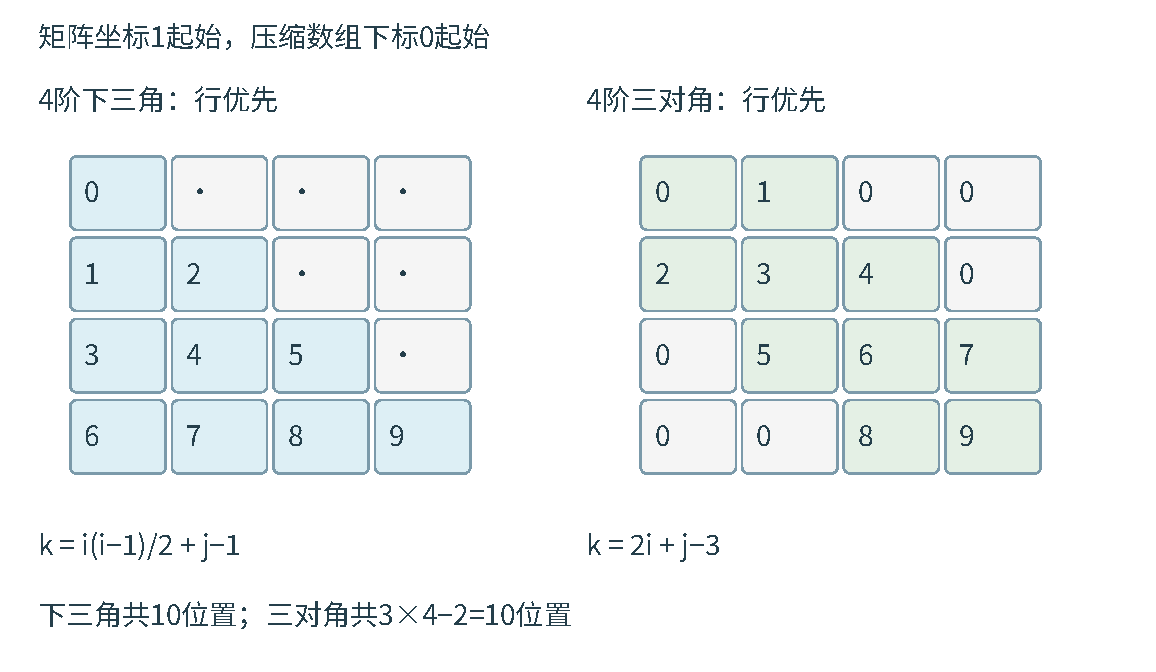
\includegraphics[width=\linewidth,height=108mm,keepaspectratio]{figures/DS03_matrix_positions.pdf}
\caption{压缩后的连续下标}\label{DS03-matrix-figure}
\end{figure}

\par\medskip\Needspace{4\baselineskip}\noindent\hypertarget{DS03-E03}{}\label{DS03-E03}\textbf{例 3-3}\par\nobreak\smallskip

100阶三对角矩阵 \(M\) 的元素 \(m_{i,j}\ (1\le i,j\le100)\) 按行优先依次压缩存入下标从0开始的一维数组 \(N\)。\(m_{30,30}\) 在 \(N\) 中的下标为（　）。

A. 86　B. 87　C. 88　D. 89

\par\medskip\Needspace{4\baselineskip}\noindent\hypertarget{DS03-E04}{}\label{DS03-E04}\textbf{例 3-4}\par\nobreak\smallskip

10\ensuremath{\times}10对称矩阵 \(M\) 的上三角元素 \(m_{i,j}\ (1\le i\le j\le10)\) 按列优先存入 C 语言一维数组 \(N\)。\(m_{7,2}\) 在 \(N\) 中的下标为（　）。

A. 15　B. 16　C. 22　D. 23

反向定位：若矩阵、数组均0起始且下三角行优先，令\(T_i=i(i+1)/2\)，找\(T_i\le k<T_{i+1}\)，再取\(j=k-T_i\)；等价地

\[i=\left\lfloor\frac{\sqrt{8k+1}-1}{2}\right\rfloor,\qquad j=k-i(i+1)/2.\]

浮点实现需用整数边界复核。三对角坐标1起始、数组0起始且\(0\le k<3n-2,n\ge2\)时：

\[i=\left\lceil\frac{k+2}{3}\right\rceil,\qquad j=k-2i+3.\]

\textbf{稀疏矩阵}非零位置无固定规律，三元组保存\texttt{(\allowbreak{}行,\allowbreak{}列,\allowbreak{}值)\allowbreak{}}并另记总行数、总列数、非零元数；全零行也计入行数。十字链表让每个非零结点同时进入行链、列链，修改须维护两组链接。坐标到压缩记录的定位依赖表示，不能直接套普通二维数组公式。
